\documentclass[11pt]{ctexart}
\usepackage[margin=2.6cm]{geometry}
\usepackage{amsmath,amssymb,amsthm}
\usepackage{booktabs,array}
\usepackage{tikz,xcolor}
\definecolor{figA}{RGB}{214,231,247}
\definecolor{figB}{RGB}{247,224,214}
\definecolor{figC}{RGB}{219,242,222}
\definecolor{figD}{RGB}{244,238,211}
\definecolor{figE}{RGB}{233,220,244}
\definecolor{figF}{RGB}{215,240,240}
\tikzset{ked/.style={line width=0.75pt},
         gone/.style={red!75!black, densely dotted, line width=1.05pt}}

\newtheorem{theorem}{定理}[section]
\newtheorem{lemma}[theorem]{引理}
\newtheorem{proposition}[theorem]{命題}
\newtheorem{corollary}[theorem]{系}
\newtheorem{conjecture}[theorem]{猜想}
\theoremstyle{definition}
\newtheorem{remark}[theorem]{註}
\newtheorem{fact}[theorem]{計算事實}
\renewcommand{\proofname}{證明}

\newcommand{\ceil}[1]{\left\lceil #1 \right\rceil}
\newcommand{\floor}[1]{\left\lfloor #1 \right\rfloor}

\title{網格圖的矩形消去數：$S(4,m)$ 至 $S(8,m)$ 的完全確定\\與一個奇偶障礙定理}
\author{（作者待填）}
\date{2026 年 7 月}

\begin{document}
\maketitle

\begin{abstract}
設 $S(n,m)$ 為使 $n\times m$ 網格圖不含任何（軸平行）矩形輪廓所需移除的最少邊數。Niu 與 Tang \cite{NT25} 確定了 $n\le 3$ 的精確值，並對 $S(5,m)$ 給出相差 $1$ 的上下界。本文完全確定 $n=4,5,6,7,8$ 的所有精確值。特別地，$S(4,m)=\ceil{30m/11}$（$m\ge 2$）：高度 $4$ 的漸近密度為 $30/11$，嚴格超過 tromino／Euler 下界的 $8/3$，且我們證明這是唯一的反常高度：對一切 $n\ge 5$ 有 $\lim_m S(n,m)/m = 2n/3$。方法上，本文的核心新工具是一個純組合的\textbf{奇偶障礙定理}：當 $nm\equiv 1\pmod 3$ 時，$S(n,m)=\ceil{2nm/3}$（即 Euler 下界緊）蘊涵 $n,m$ 皆為偶數。此定理一舉給出 $5\times(3k{+}2)$、$7\times(3k{+}1)$、$8\times(6t{+}5)$ 三族「Euler${}+1$」下界的純人工證明，並解釋了 Golomb 型構造為何恰在 $2^k\times 2^k$ 可行。我們同時以帶介面條件的疊置引理修補並推廣 \cite{NT25} 定理 3（去除 $m\ge n\ge 8$ 之限制），並為 $S(4,m)\ge 30m/11$ 給出一個可獨立核驗的靜態位勢證書。所有計算性結論均附確定性有限證書與多重獨立交叉驗證。
\end{abstract}

\section{引言}

在 $n\times m$ 網格圖（$(n{+}1)(m{+}1)$ 個頂點、$2nm+n+m$ 條單位邊）中，一個\emph{矩形輪廓}指某個格點矩形 $[j_1,j_2]\times[i_1,i_2]$（$i_1<i_2$，$j_1<j_2$）之邊界迴路。稱邊集 $A$ 為\emph{矩形消去集}，若移除 $A$ 後殘圖不含任何矩形輪廓；$S(n,m)$ 為其最小基數。此量由 Niu--Tang \cite{NT25} 系統研究：他們給出 $S(1,m)=m$、$S(2,m)=\ceil{3m/2}$、$S(3,m)=2m+1$，證明一般下界 $S(n,m)\ge\ceil{2nm/3}$（$3\mid nm$ 時再加 $1$；見註~\ref{rem:errata}），對 $m\equiv 0\pmod 3$ 確定 $S(5,m)=10m/3+1$，對其餘餘數給出相差 $1$ 的上下界，並藉 Golomb 的殘缺 tromino 鑲嵌 \cite{Golomb54} 得 $S(2^k,2^k)=(2\cdot 4^k+1)/3$。

本文的貢獻如下。

\smallskip
\noindent\textbf{(A) 精確值。}我們完全確定 $n=4,5,6,7,8$ 之 $S(n,m)$（定理~\ref{thm:n4}--\ref{thm:n8}）。其中 $S(5,m)$ 關閉了 \cite{NT25} 的兩個差 $1$ 缺口：$m\equiv 1\pmod 3$ 時其\emph{下界}正確（上界可省 $1$），$m\equiv 2$ 時其\emph{上界}正確（下界需加 $1$）。最出乎意料者為
\[
  S(4,m)=\ceil{30m/11}\qquad(m\ge 2):
\]
高度 $4$ 的每列密度為 $30/11\approx 2.727$，嚴格大於 tromino 下界的 $8/3$；結構上，最優解被迫以每 $11$ 列 $2$ 個的固定速率使用四格骨牌面（$12$ 個 L 形 tromino 面加 $2$ 個非矩形四格骨牌面覆蓋每週期的 $44$ 格）。

\smallskip
\noindent\textbf{(B) 奇偶障礙定理。}定理~\ref{thm:parity}：若 $nm\equiv 1\pmod 3$ 且 $S(n,m)=\ceil{2nm/3}$，則 $n$ 與 $m$ 皆為偶數。其證明為純組合論證（約兩頁），核心是把 Euler-緊解剛性化為「肘部組態」（引理~\ref{lem:rigid}、\ref{lem:elbow}）後，對頂端兩行做一次精確的計數（引理~\ref{lem:band}），再讀出第 $1$ 行與第 $n$ 行胞腔方程的 mod $2$ 資訊。由此，$S(5,3k{+}2)$、$S(7,3k{+}1)$、$S(8,6t{+}5)$ 三族的「Euler${}+1$」下界皆獲純人工證明，且 $n=4$、$m\equiv 1\pmod 6$ 時亦然。

\smallskip
\noindent\textbf{(C) 密度定理與一般上界。}定理~\ref{thm:density}：$\delta(n):=\lim_m S(n,m)/m$ 滿足 $\delta(n)=2n/3$ 對一切 $n\ge 5$，而 $\delta(4)=30/11$ 為（除平凡之 $n=1,2$ 外）唯一反常。我們並以帶介面條件 $(*)$ 的疊置引理（引理~\ref{lem:stack}）補嚴 \cite{NT25} 定理 3 的層間論證，將其自 $m\ge n\ge 8$ 推廣到所有 $n\ge 3$、所有 $m\ge 2$，且證明條件 $(*)$ 對高度 $3,4,5$ 之帶狀最優解\emph{無額外代價}。

\smallskip
\noindent\textbf{(D) 證明標準之宣告。}本文採兩級標準並逐一標註：\emph{人證}（不依賴機器）與\emph{有限證書}（由確定性有限計算建立、附靜態資料可獨立復核；見第~\ref{sec:scan} 節之引理~\ref{lem:exact}--\ref{lem:cert} 與第~\ref{sec:comp} 節）。特別地：$n=5,6,7,8$ 的\emph{全部下界}均為人證；$S(4,m)\ge 30m/11$ 由一張 $522$ 行的靜態位勢表配三族有限不等式核驗（命題~\ref{prop:psi}），其數學論證僅五行；各上界由機器構造之顯式解（每個皆經獨立暴力驗證器復核）與週期性證書（引理~\ref{lem:cert}）承擔。

\section{預備與 Euler 型下界}\label{sec:prelim}

胞腔記為 $(r,c)$，$1\le r\le n$（自上而下）、$1\le c\le m$。水平線 $i=0,\dots,n$；豎直線 $j=0,\dots,m$。$h(i,c)$ 表第 $i$ 條水平線上跨第 $c$ 列之邊；$v(r,j)$ 表第 $j$ 條豎直線上跨第 $r$ 行之邊。矩形 $(i_1,i_2,j_1,j_2)$ 之輪廓為
$\{h(i_1,c),h(i_2,c): j_1<c\le j_2\}\cup\{v(r,j_1),v(r,j_2): i_1<r\le i_2\}$。
移除集 $A$ 合法即每個輪廓與 $A$ 相交。稱網格外緣上的邊為\emph{周界邊}。

以下面結構引理是全文的幾何基礎。移除 $A$ 後的平面圖記為 $G'$（保留全部頂點）；$G'$ 的面即 $\mathbb R^2\setminus G'$ 的連通分支。對每個面 $F$，其\emph{胞腔集}為內部含於 $F$ 的單位胞腔全體。

\begin{lemma}[面結構]\label{lem:face}
設 $A$ 為任意移除集。則
\emph{(i)} 兩胞腔若共用一條被移除的邊，則屬同一面；
\emph{(ii)} 反之，同一面之任兩胞腔可由一列胞腔相連，其中相鄰兩項共用一條被移除的\emph{內部}邊；且某胞腔屬外面若且唯若它可經此種鏈接到某個帶有被移除\emph{周界}邊的胞腔（含長度零之鏈）；
\emph{(iii)} 若某有界面之胞腔集恰構成一個 $p\times q$ 矩形區域，則該矩形之輪廓全數保留於 $G'$。因而合法之 $A$ 下：每個有界面之胞腔數 $\ge 3$，且胞腔數為 $3$ 者必為 L 形 tromino。
\end{lemma}

\begin{proof}
(i) 顯然。(ii) 取面內連接兩胞腔內點之道路 $\gamma$。$G'$ 為閉集，網格頂點為有限點集；平面開連通集去除有限多點仍道路連通，故可擾動 $\gamma$ 使其避開所有頂點與保留邊，於是 $\gamma$ 穿越網格線僅發生於被移除邊之內點：每次穿越即在共用該邊之兩胞腔間移動（周界邊之穿越則在邊界胞腔與無界區域間移動）。讀出 $\gamma$ 依序訪問之胞腔即得所需之鏈。(iii) 設輪廓上某邊 $e$ 被移除：若 $e$ 為內部邊，則由 (i)，$e$ 外側胞腔與面同屬一面，與胞腔集恰為該矩形矛盾；若 $e$ 為周界邊，則面併入無界區域，與有界矛盾。故輪廓全保留。合法性排除矩形面；胞腔數 $1,2$ 之面為 $1\times1,1\times2$ 矩形，胞腔數 $3$ 之直 tromino 為 $1\times 3$ 矩形，均被排除。
\end{proof}

\begin{theorem}[Euler 型下界；本質見 \cite{NT25}]\label{thm:euler}
$S(n,m)\ge\ceil{2nm/3}$；若 $3\mid nm$，則 $S(n,m)\ge 2nm/3+1$。
\end{theorem}

\begin{proof}
設 $A$ 合法，$k=|A|$，$G'$ 有 $c$ 個分支、$B$ 個有界面。Euler 公式（含分支修正）給
$(n{+}1)(m{+}1)-(2nm{+}n{+}m-k)+(B{+}1)=1+c$，即 $k=nm-1+c-B$。由引理~\ref{lem:face}(iii) 各有界面胞腔數 $\ge 3$，故 $B\le\floor{nm/3}$，得 $k\ge nm-\floor{nm/3}=\ceil{2nm/3}$。若 $3\mid nm$ 且 $k=2nm/3$，則 $c=1$、$B=nm/3$、諸面胞腔數恰為 $3$ 且覆蓋全部胞腔；於是每條周界邊分隔一有界面與外面，必保留，整個 $n\times m$ 輪廓完好，矛盾。
\end{proof}

\begin{remark}\label{rem:errata}
\cite{NT25} 中「$+1$」之條件寫作 $n\equiv 0\pmod 3$；如上證所示（亦如其定理 5 中 $m\equiv 0$ 之用法），正確條件為 $3\mid nm$。
\end{remark}

\section{掃描形式化與有限證書}\label{sec:scan}

本節建立「對\emph{所有} $m$」之計算性斷言的嚴格意涵。固定 $n$。自左而右掃描豎直線；\emph{狀態}為行對 $(i_1,i_2)$（$0\le i_1<i_2\le n$，共 $\binom{n+1}{2}$ 個）之布林向量：
\[
\mathrm{live}[i_1,i_2]=1 \iff \exists\, j_1\le j:\ v(r,j_1)\ \text{全保留}\ (i_1<r\le i_2)\ \text{且}\ h(i_1,c),h(i_2,c)\ \text{全保留}\ (j_1<c\le j).
\]
處理第 $c$ 列時選取保留之水平邊集 $H\subseteq\{0,\dots,n\}$ 與新豎線之保留豎邊集 $V\subseteq\{1,\dots,n\}$；記 $K_H$ 為兩端線皆屬 $H$ 之行對集、$N_V$ 為 $(i_1,i_2]$ 段全含於 $V$ 之行對集。若 $(\mathrm{live}\cap K_H)\cap N_V\ne\varnothing$ 則發生\emph{閉合}（非法）；否則 $\mathrm{live}'=(\mathrm{live}\cap K_H)\cup N_V$。代價為本列被移除邊數。

\begin{lemma}[正確性]\label{lem:exact}
移除集與掃描過程一一對應；$A$ 合法 $\iff$ 全程無閉合。且任一前綴之後的可行延拓集合與最小延拓代價僅依賴當前 $\mathrm{live}$。
\end{lemma}

\begin{proof}
若矩形 $(i_1,i_2,j_1,j_2)$ 於 $A$ 下存活：於線 $j_1$ 該行對之 $\mathrm{live}$ 置真；頂底兩線於 $(j_1,j_2]$ 完好使其持續為真；於線 $j_2$ 右側整段保留即觸發閉合。反之，閉合發生時由 $\mathrm{live}$ 之定義存在見證 $j_1<j_2$ 使該矩形完整。末句成立係因未來之閉合條件僅經 $\mathrm{live}$ 讀取歷史，且 $\mathrm{live}$ 之轉移僅依賴當前值與新選擇。
\end{proof}

\begin{lemma}[支配剪枝]\label{lem:prune}
以「最小代價達成」為值之狀態前沿中，若 $\mathrm{mask}\subseteq\mathrm{mask}'$ 且代價不大，刪去 $(\mathrm{mask}',\cdot)$ 不改變任何寬度之最優值；且剪枝後之前沿轉移為確定性映射。
\end{lemma}

\begin{proof}
相同選擇下，子集狀態之後繼仍為子集，且合法選擇集合更大；對剩餘列數歸納即得值函數對 $\mathrm{mask}$ 單調。轉移之確定性由「先窮舉、後以固定規則剪枝」立得。
\end{proof}

\begin{lemma}[週期性證書]\label{lem:cert}
記 $\widehat F_j$ 為寬度 $j$ 時之\emph{規範化}前沿（各代價減去最小值）。若 $\widehat F_{m_1}=\widehat F_{m_2}$（$m_1<m_2$），則對一切 $m\ge m_1$：$S(n,m+p)=S(n,m)+\Delta$，其中 $p=m_2-m_1$、$\Delta=S(n,m_2)-S(n,m_1)$。
\end{lemma}

\begin{proof}
由引理~\ref{lem:prune}，$\widehat F_{j}\mapsto\widehat F_{j+1}$ 為確定性映射，且 $S(n,j)$ 之逐列增量僅由 $\widehat F_j$ 決定；相同之規範化前沿故產生相同之後續增量序列。
\end{proof}

計算得之證書：$n=4:(m_1,m_2,\Delta)=(8,19,30)$；$n=5:(10,13,10)$；$n=6:(5,7,8)$；$n=7:(7,13,28)$；$n=8:(10,16,32)$。配合小寬度之直接計算值，即得第~\ref{sec:exact} 節諸公式對\emph{所有} $m$ 成立。

\section{剛性結構：肘部組態}\label{sec:rigid}

\begin{lemma}[剛性]\label{lem:rigid}
設 $nm\equiv 1\pmod 3$ 且 $A$ 為恰含 $\ceil{2nm/3}=(2nm+1)/3$ 條邊之合法移除集。則：$G'$ 連通；有界面恰為 $(nm-1)/3$ 個 L 形 tromino，覆蓋除一個邊界胞腔 $x$ 外之全部胞腔；$x$ 屬外面；$A$ 恰由「$x$ 的一條周界邊 $e_x$」與「每個 tromino 的兩條內部邊」組成（全網格僅此一條周界邊被移除）。
\end{lemma}

\begin{proof}
沿定理~\ref{thm:euler} 之記號：$k=nm-1+c-B\;$且$\;B\le\floor{nm/3}=(nm-1)/3$，等號迫使 $c=1$、$B=(nm-1)/3$。諸面胞腔數 $\ge3$ 且總和 $\le nm$；若總和 $=nm$ 則如前周界完好而矛盾，故總和 $\le nm-1=3B$，於是各面胞腔數恰為 $3$（皆 L 形）且恰有一胞腔 $x$ 不被覆蓋，$x$ 屬外面。被移除的\emph{內部}邊兩側胞腔同面（引理~\ref{lem:face}(i)）：兩側均為 tromino 胞腔時屬同一 tromino；不可能兩側皆屬外面（僅 $x$ 未覆蓋）。反之，每個 L 形 tromino 之三胞腔須以被移除之共用邊相連（引理~\ref{lem:face}(ii)），其胞腔相鄰圖為兩邊之路徑，故其\emph{兩條}內部共用邊皆被移除。於是內部被移除邊恰 $2(nm-1)/3$ 條，周界被移除邊恰 $(2nm+1)/3-2(nm-1)/3=1$ 條，記為 $e_x$；其內側胞腔併入外面故未被覆蓋，即為 $x$。最後，$x$ 屬外面，由引理~\ref{lem:face}(ii) 存在以被移除內部邊相連、終於帶被移除周界邊之胞腔之鏈；鏈上諸胞腔皆屬外面故未被覆蓋，鏈長必為零，即 $e_x$ 為 $x$ 自身之周界邊。
\end{proof}

\begin{lemma}[肘部結構]\label{lem:elbow}
剛性組態中，每個 tromino 之三胞腔恰為某內部格點（其\emph{中心}）周圍四胞腔中之三個；其兩條被移除邊為該格點四條關聯邊中相鄰之兩條（一橫一豎），於中心處構成一「肘」。相異 tromino 之中心相異。依缺失象限分類：\emph{上型}（佔上兩胞腔；移除中心之上邊）、\emph{下型}（移除下邊）；同時亦為\emph{左型}（佔左兩胞腔；移除左邊）或\emph{右型}（移除右邊）。
\end{lemma}

\begin{proof}
L 形 tromino 之包絡盒為 $2\times2$ 缺一角；其兩條內部邊即盒中心格點之兩條關聯邊（逐一檢視四種朝向），且恰一橫一豎。兩 tromino 共中心則共用被移除邊或共用胞腔，皆不可能。
\end{proof}

對水平線 $\ell\in[1,n-1]$，記中心落於線 $\ell$ 之 tromino 數為 $t_\ell=u_\ell+d_\ell$（上型 $u_\ell$、下型 $d_\ell$）；對豎直線 $c\in[1,m-1]$ 同理記 $\lambda_c$（左型）、$\rho_c$（右型）。令 $\varepsilon_r=[\,x\text{ 在第 }r\text{ 行}\,]$。第 $r$ 行之胞腔由線 $r{-}1$ 與線 $r$ 之中心覆蓋（約定 $t_0=t_n=0$）：
\begin{equation}\label{eq:row}
u_{r-1}+2d_{r-1}+2u_r+d_r \;=\; m-\varepsilon_r\qquad(1\le r\le n),
\end{equation}
豎直方向有對稱之\emph{列方程}。圖~\ref{fig:rigid44} 展示一個 $4\times4$ 之剛性組態（$S(4,4)=11$ 之最優解）：五個 tromino、其肘部中心（黑點）、開放胞腔 $x$。

\begin{figure}[htbp]\centering
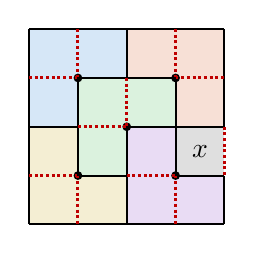
\begin{tikzpicture}[scale=0.62]
\fill[figA] (0,3) rectangle (1,4);
\fill[figA] (1,3) rectangle (2,4);
\fill[figA] (0,2) rectangle (1,3);
\fill[figB] (2,3) rectangle (3,4);
\fill[figB] (3,3) rectangle (4,4);
\fill[figB] (3,2) rectangle (4,3);
\fill[figC] (1,2) rectangle (2,3);
\fill[figC] (2,2) rectangle (3,3);
\fill[figC] (1,1) rectangle (2,2);
\fill[figD] (0,1) rectangle (1,2);
\fill[figD] (0,0) rectangle (1,1);
\fill[figD] (1,0) rectangle (2,1);
\fill[figE] (2,1) rectangle (3,2);
\fill[figE] (2,0) rectangle (3,1);
\fill[figE] (3,0) rectangle (4,1);
\fill[gray!25] (3,1) rectangle (4,2);
\node at (3.5,1.5) {$x$};
\fill[black] (1,3) circle (0.09);
\fill[black] (3,3) circle (0.09);
\fill[black] (2,2) circle (0.09);
\fill[black] (1,1) circle (0.09);
\fill[black] (3,1) circle (0.09);
\draw[ked] (0,4) -- (4,4);
\draw[ked] (1,3) -- (3,3);
\draw[ked] (0,2) -- (1,2);
\draw[ked] (2,2) -- (4,2);
\draw[ked] (1,1) -- (2,1);
\draw[ked] (3,1) -- (4,1);
\draw[ked] (0,0) -- (4,0);
\draw[ked] (0,4) -- (0,0);
\draw[ked] (1,3) -- (1,1);
\draw[ked] (2,4) -- (2,3);
\draw[ked] (2,2) -- (2,0);
\draw[ked] (3,3) -- (3,1);
\draw[ked] (4,4) -- (4,2);
\draw[ked] (4,1) -- (4,0);
\draw[gone] (0,3) -- (1,3);
\draw[gone] (3,3) -- (4,3);
\draw[gone] (1,2) -- (2,2);
\draw[gone] (0,1) -- (1,1);
\draw[gone] (2,1) -- (3,1);
\draw[gone] (1,4) -- (1,3);
\draw[gone] (3,4) -- (3,3);
\draw[gone] (2,3) -- (2,2);
\draw[gone] (4,2) -- (4,1);
\draw[gone] (1,1) -- (1,0);
\draw[gone] (3,1) -- (3,0);
\end{tikzpicture}
\caption{$4\times4$ 之剛性組態（Euler-緊，$11$ 條邊；紅點線為被移除邊）。五個 L 形 tromino 面各以底色標示，黑點為其肘部中心；$x=(3,4)$ 為開放邊界胞腔，其周界邊 $v(3,4)$ 為全組態唯一被移除之周界邊。此例中 $d_1=u_3=\rho_1=0$、$\lambda_3=1$（$x$ 在第 $m$ 列，屬引理~\ref{lem:band} 允許之例外），且 $n=m=4$ 皆偶，與定理~\ref{thm:parity} 一致。}
\label{fig:rigid44}
\end{figure}

\section{奇偶障礙定理}\label{sec:parity}

以下設 $n,m\ge 3$，$nm\equiv1\pmod3$，並固定一剛性組態（引理~\ref{lem:rigid}）。

\begin{lemma}[頂帶引理]\label{lem:band}
令 $\chi=[\,e_x\in\{v(1,0),v(2,0),v(1,m),v(2,m)\}\,]$。則
\[
d_1\;\le\;\varepsilon_1+\chi-\varepsilon_2 .
\]
特別地，若 $x$ 不在第 $1$ 行，則 $d_1=0$。上下鏡射給出對稱結論：若 $x$ 不在第 $n$ 行，則 $u_{n-1}=0$。
\end{lemma}

\begin{proof}
考察行對 $(0,2)$ 之全部矩形 $(0,2,j_1,j_2)$。稱豎直線 $j$ 為\emph{受刺}，若 $v(1,j)$ 或 $v(2,j)$ 被移除。由引理~\ref{lem:elbow} 之分類：$v(1,j)$ 被移除 $\iff$ 線 $1$ 有上型中心於列 $j$；$v(2,j)$ 被移除 $\iff$ 線 $1$ 有下型中心於 $j$ 或線 $2$ 有上型中心於 $j$（線 $0$ 無中心）。故內部受刺線之列集合含於「線 $1$ 之全部中心列」$\cup$「線 $2$ 之上型中心列」，基數 $\le t_1+u_2$；邊界線 $j\in\{0,m\}$ 受刺唯當 $e_x$ 為第 $1$ 或 $2$ 行之豎周界邊，共 $\le\chi$ 條。於是受刺線總數 $P\le t_1+u_2+\chi$，未受刺線數 $U=(m{+}1)-P\ge m+1-t_1-u_2-\chi$。

未受刺線兩兩構成之矩形須由\emph{頂邊或底邊}破壞：即線 $0$ 或線 $2$ 於 $(j_1,j_2]$ 內有被移除之水平邊。線 $0$ 上被移除邊唯 $e_x$（此時 $x$ 在第 $1$ 行），至多 $\varepsilon_1$ 條；線 $2$ 上被移除邊恰為線 $2$ 諸中心各貢獻一條（左型於中心列、右型於中心列 $+1$；相異 tromino 之被移除邊相異），共 $t_2$ 條（$n\ge3$ 保證線 $2$ 非周界，故無 $e_x$ 之干擾）。設未受刺線為 $j^{(1)}<\dots<j^{(U)}$；諸區間 $(j^{(s)},j^{(s+1)}]$ 兩兩不交且每個至少須含一條上述分隔邊，故
\[
U-1\;\le\;t_2+\varepsilon_1 .
\]
合併兩式：$m-t_1-u_2-\chi\le t_2+\varepsilon_1$，即 $m\le t_1+u_2+t_2+\varepsilon_1+\chi$。以第 $2$ 行胞腔方程 \eqref{eq:row}（$r=2$）$m=u_1+2d_1+2u_2+d_2+\varepsilon_2$ 代入並用 $t_1=u_1+d_1$、$t_2=u_2+d_2$ 化簡，得 $d_1+\varepsilon_2\le\varepsilon_1+\chi$。

末句：若 $x$ 不在第 $1$ 行而 $\chi=1$，則 $e_x\in\{v(2,0),v(2,m)\}$，故 $x\in\{(2,1),(2,m)\}$、$\varepsilon_2=1$，於是 $d_1\le0+1-1=0$；$\chi=0$ 時直接 $d_1\le-\varepsilon_2\le0$。
\end{proof}

\begin{theorem}[奇偶障礙]\label{thm:parity}
設 $n,m\ge3$ 且 $nm\equiv1\pmod3$。若 $S(n,m)=\ceil{2nm/3}$，則 $n$ 與 $m$ 皆為偶數。
\end{theorem}

\begin{proof}
取剛性組態。若 $x$ 不在第 $1$ 行：由引理~\ref{lem:band} 得 $d_1=0$，又 $\varepsilon_1=0$，故 \eqref{eq:row}（$r=1$）讀作 $m=2u_1$，$m$ 為偶。否則 $x$ 在第 $1$ 行、必不在第 $n$ 行：對稱地 $u_{n-1}=0$、$\varepsilon_n=0$，\eqref{eq:row}（$r=n$）讀作 $m=2d_{n-1}$，$m$ 為偶。將整個組態轉置（tromino、周界邊、矩形輪廓皆保持），對 $m\times n$ 板重複上述論證即得 $n$ 為偶。
\end{proof}

\begin{corollary}\label{cor:families}
以下下界成立（皆為人證；配合第~\ref{sec:exact} 節之上界即為等式）：
\emph{(i)} $S(5,3k{+}2)\ge 10k+8$（$k\ge0$）；
\emph{(ii)} $S(7,3k{+}1)\ge 14k+6$（$k\ge1$）；
\emph{(iii)} $S(8,m)\ge (16m+4)/3$ 當 $m\equiv5\pmod6$；
\emph{(iv)} $S(4,m)\ge\ceil{8m/3}+1$ 當 $m\equiv1\pmod6$。
\end{corollary}

\begin{proof}
各情形 $nm\equiv1\pmod3$ 而兩邊長非皆偶：(i)(ii) 中 $n$ 為奇；(iii)(iv) 中 $m$ 為奇。由定理~\ref{thm:parity}，Euler 下界不可達，故至少再加 $1$。
\end{proof}

\begin{remark}
定理~\ref{thm:parity} 亦回溯性地解釋了 \cite{NT25,Golomb54} 之 $S(2^k,2^k)=(2\cdot4^k+1)/3$：兩邊長皆偶，奇偶障礙不生效。必要條件之外，充分性見第~\ref{sec:open} 節猜想~\ref{conj:even}。
\end{remark}

\section{各高度之精確值}\label{sec:exact}

以下五個定理之\emph{下界}來源標於各式之後；\emph{上界}一律由機器構造之顯式解承擔：對每個計算範圍內之 $m$，動態規劃回溯出具體移除集並經獨立暴力驗證器逐矩形復核（圖~\ref{fig:sol413}、\ref{fig:sol58} 為兩例），對一切 $m$ 之存在性則由引理~\ref{lem:cert} 之證書保證。

\begin{theorem}[$n=4$]\label{thm:n4}
$S(4,1)=4$；對一切 $m\ge2$，$S(4,m)=\ceil{30m/11}$。
\end{theorem}

下界即命題~\ref{prop:psi}；另見系~\ref{cor:families}(iv)（$m\equiv1\pmod6$ 時之人證，於 $m\in\{7,13,19\}$ 恰為緊）。

\begin{proposition}[位勢證書]\label{prop:psi}
存在函數 $\Psi:\mathcal R\to\{0,1,\dots,46\}$（$\mathcal R$ 為 $n=4$ 掃描之全部 $522$ 個可達狀態；資料檔 \texttt{psi4.json}），滿足
\emph{(C1)} $\Psi\ge0$；
\emph{(C2)} 對每個初始選擇 $V_0$：$\Psi(\mathrm{live}_0)\le 11\cdot(\text{第 }0\text{ 線移除數})$；
\emph{(C3)} 對每個可達狀態 $s$ 與每個合法列選擇 $(H,V)$：$\Psi(s')\le\Psi(s)+11\cdot(\text{本列移除數})-30$。
凡此三族有限不等式已逐一核驗。由之，對一切 $m\ge1$：$S(4,m)\ge 30m/11$，故 $S(4,m)\ge\ceil{30m/11}$。
\end{proposition}

\begin{proof}[證明（給定 C1--C3）]
任一合法解對應軌跡 $s_0,s_1,\dots,s_m$（引理~\ref{lem:exact}）。記其總移除數為 $K$，則
\[
11K\;\overset{\text{C2,C3}}{\ge}\;\Psi(s_0)+\sum_{i=1}^{m}\bigl(30+\Psi(s_i)-\Psi(s_{i-1})\bigr)\;=\;30m+\Psi(s_m)\;\overset{\text{C1}}{\ge}\;30m. \qedhere
\]
\end{proof}

\begin{remark}
每 $11$ 列恰花 $30$ 條邊之結構解讀：設一週期內部由 $t$ 個 tromino 面與 $q$ 個非矩形四格骨牌面構成（後者移除 $3$ 條內部邊），則 $3t+4q=44$、$2t+3q=30$，解得 $t=12$、$q=2$：高度 $4$ 之最優解被迫以固定速率使用四格骨牌面，此即 $8/3$ 密度不可維持之組合原因；$\Psi$ 正是此「欠賬」之離散對偶量化。
\end{remark}

\begin{theorem}[$n=5$；關閉 \cite{NT25} 之缺口]\label{thm:n5}
$S(5,1)=5$；對 $m\ge2$：
\[
S(5,m)=\begin{cases}
\dfrac{10m}{3}+1, & m\equiv0\pmod3\quad(\text{下界：定理~\ref{thm:euler}；亦見 \cite{NT25}}),\\[4pt]
\dfrac{10m+2}{3}, & m\equiv1\pmod3\quad(\text{下界：定理~\ref{thm:euler}}),\\[4pt]
\dfrac{10m+4}{3}, & m\equiv2\pmod3\quad(\text{下界：系~\ref{cor:families}(i)}).
\end{cases}
\]
特別地，$m\equiv1$ 時 \cite{NT25} 之下界正確而其上界可改進 $1$；$m\equiv2$ 時其上界正確而其下界須加 $1$。
\end{theorem}

\begin{theorem}[$n=6$]\label{thm:n6}
$S(6,1)=6$；對一切 $m\ge2$，$S(6,m)=4m+1$（下界：定理~\ref{thm:euler}，因 $3\mid6m$ 恆成立）。
\end{theorem}

\begin{theorem}[$n=7$]\label{thm:n7}
$S(7,1)=7$、$S(7,2)=11$；對 $m\ge3$：
\[
S(7,m)=\begin{cases}
\dfrac{14m}{3}+1, & m\equiv0\pmod3\quad(\text{下界：定理~\ref{thm:euler}}),\\[4pt]
\dfrac{14m+4}{3}, & m\equiv1\pmod3\quad(\text{下界：系~\ref{cor:families}(ii)}),\\[4pt]
\dfrac{14m+2}{3}, & m\equiv2\pmod3\quad(\text{下界：定理~\ref{thm:euler}}).
\end{cases}
\]
\end{theorem}

\begin{theorem}[$n=8$]\label{thm:n8}
$S(8,1)=8$、$S(8,2)=12$；對 $m\ge3$：
\[
S(8,m)=\begin{cases}
\dfrac{16m}{3}+1, & m\equiv0\pmod3,\\[4pt]
\dfrac{16m+2}{3}, & m\equiv1\pmod3,\\[4pt]
\dfrac{16m+1}{3}+[\,m\text{ 為奇}\,], & m\equiv2\pmod3\quad(\text{奇之下界：系~\ref{cor:families}(iii)}).
\end{cases}
\]
\end{theorem}

\begin{remark}
定理~\ref{thm:n8} 之 $m\equiv2\pmod3$ 分支呈現\emph{奇偶分裂}：$m$ 偶（$m=8,14,20,\dots$）時 Euler 下界緊（剛性組態存在；$8\times8$ 即 Golomb 情形；殘缺板 tromino 鑲嵌之經典脈絡見 \cite{CJ86}），$m$ 奇時由奇偶障礙加 $1$。這說明「$nm\bmod3$ 決定 $\varepsilon(n,m):=S-\ceil{2nm/3}$」之樸素統一律不成立，正確之刻畫繫於剛性組態之存在性。彙總（$m\ge3$，小例外除外）：$nm\equiv0\pmod3$ 時 $\varepsilon=1$；$nm\equiv2$ 時 $\varepsilon=0$；$nm\equiv1$ 時 $\varepsilon=1$ 若 $n,m$ 非皆偶（定理~\ref{thm:parity}），而 $n=8$ 之資料顯示皆偶時 $\varepsilon=0$（$m\ge8$）。
\end{remark}

計算值總表（$m\le 14$；更大之 $m$ 由諸公式與證書給出）：
\begin{center}\small
\begin{tabular}{c|cccccccccccccc}
\toprule
$m$ & 1&2&3&4&5&6&7&8&9&10&11&12&13&14\\
\midrule
$S(4,m)$ & 4&6&9&11&14&17&$20$&22&25&$28$&30&33&$36$&$39$\\
$S(5,m)$ & 5&8&11&14&18&21&24&28&31&34&38&41&44&48\\
$S(6,m)$ & 6&9&13&17&21&25&29&33&37&41&45&49&53&57\\
$S(7,m)$ & 7&11&15&20&24&29&34&38&43&48&52&57&62&66\\
$S(8,m)$ & 8&12&17&22&28&33&38&43&49&54&60&65&70&75\\
\bottomrule
\end{tabular}
\end{center}

\begin{figure}[htbp]\centering
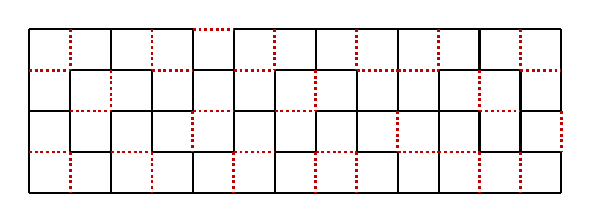
\begin{tikzpicture}[scale=0.52]
\draw[ked] (0,4) -- (4,4);
\draw[ked] (5,4) -- (13,4);
\draw[ked] (1,3) -- (3,3);
\draw[ked] (4,3) -- (5,3);
\draw[ked] (6,3) -- (8,3);
\draw[ked] (10,3) -- (12,3);
\draw[ked] (0,2) -- (1,2);
\draw[ked] (2,2) -- (4,2);
\draw[ked] (5,2) -- (6,2);
\draw[ked] (7,2) -- (11,2);
\draw[ked] (12,2) -- (13,2);
\draw[ked] (1,1) -- (2,1);
\draw[ked] (3,1) -- (5,1);
\draw[ked] (6,1) -- (7,1);
\draw[ked] (8,1) -- (9,1);
\draw[ked] (11,1) -- (13,1);
\draw[ked] (0,0) -- (13,0);
\draw[ked] (0,4) -- (0,0);
\draw[ked] (1,3) -- (1,1);
\draw[ked] (2,4) -- (2,3);
\draw[ked] (2,2) -- (2,0);
\draw[ked] (3,3) -- (3,1);
\draw[ked] (4,4) -- (4,2);
\draw[ked] (4,1) -- (4,0);
\draw[ked] (5,4) -- (5,1);
\draw[ked] (6,3) -- (6,0);
\draw[ked] (7,4) -- (7,3);
\draw[ked] (7,2) -- (7,1);
\draw[ked] (8,3) -- (8,1);
\draw[ked] (9,4) -- (9,2);
\draw[ked] (9,1) -- (9,0);
\draw[ked] (10,3) -- (10,0);
\draw[ked] (11,4) -- (11,3);
\draw[ked] (11,2) -- (11,1);
\draw[ked] (12,3) -- (12,1);
\draw[ked] (13,4) -- (13,2);
\draw[ked] (13,1) -- (13,0);
\draw[gone] (4,4) -- (5,4);
\draw[gone] (0,3) -- (1,3);
\draw[gone] (3,3) -- (4,3);
\draw[gone] (5,3) -- (6,3);
\draw[gone] (8,3) -- (9,3);
\draw[gone] (9,3) -- (10,3);
\draw[gone] (12,3) -- (13,3);
\draw[gone] (1,2) -- (2,2);
\draw[gone] (4,2) -- (5,2);
\draw[gone] (6,2) -- (7,2);
\draw[gone] (11,2) -- (12,2);
\draw[gone] (0,1) -- (1,1);
\draw[gone] (2,1) -- (3,1);
\draw[gone] (5,1) -- (6,1);
\draw[gone] (7,1) -- (8,1);
\draw[gone] (9,1) -- (10,1);
\draw[gone] (10,1) -- (11,1);
\draw[gone] (1,4) -- (1,3);
\draw[gone] (3,4) -- (3,3);
\draw[gone] (6,4) -- (6,3);
\draw[gone] (8,4) -- (8,3);
\draw[gone] (10,4) -- (10,3);
\draw[gone] (12,4) -- (12,3);
\draw[gone] (2,3) -- (2,2);
\draw[gone] (7,3) -- (7,2);
\draw[gone] (11,3) -- (11,2);
\draw[gone] (4,2) -- (4,1);
\draw[gone] (9,2) -- (9,1);
\draw[gone] (13,2) -- (13,1);
\draw[gone] (1,1) -- (1,0);
\draw[gone] (3,1) -- (3,0);
\draw[gone] (5,1) -- (5,0);
\draw[gone] (7,1) -- (7,0);
\draw[gone] (8,1) -- (8,0);
\draw[gone] (11,1) -- (11,0);
\draw[gone] (12,1) -- (12,0);
\end{tikzpicture}
\caption{$S(4,13)=36$ 之最優解（$=\ceil{390/11}$，超出 Euler 下界 $35$）。紅點線為被移除邊；本解經獨立暴力驗證器復核。}
\label{fig:sol413}
\end{figure}

\begin{figure}[htbp]\centering
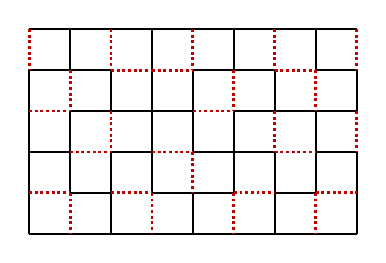
\begin{tikzpicture}[scale=0.52]
\draw[ked] (0,5) -- (8,5);
\draw[ked] (0,4) -- (2,4);
\draw[ked] (4,4) -- (6,4);
\draw[ked] (7,4) -- (8,4);
\draw[ked] (1,3) -- (4,3);
\draw[ked] (5,3) -- (8,3);
\draw[ked] (0,2) -- (1,2);
\draw[ked] (2,2) -- (3,2);
\draw[ked] (4,2) -- (6,2);
\draw[ked] (7,2) -- (8,2);
\draw[ked] (1,1) -- (2,1);
\draw[ked] (3,1) -- (5,1);
\draw[ked] (6,1) -- (7,1);
\draw[ked] (0,0) -- (8,0);
\draw[ked] (0,4) -- (0,0);
\draw[ked] (1,5) -- (1,4);
\draw[ked] (1,3) -- (1,1);
\draw[ked] (2,4) -- (2,3);
\draw[ked] (2,2) -- (2,0);
\draw[ked] (3,5) -- (3,1);
\draw[ked] (4,4) -- (4,2);
\draw[ked] (4,1) -- (4,0);
\draw[ked] (5,5) -- (5,4);
\draw[ked] (5,3) -- (5,1);
\draw[ked] (6,4) -- (6,3);
\draw[ked] (6,2) -- (6,0);
\draw[ked] (7,5) -- (7,4);
\draw[ked] (7,3) -- (7,1);
\draw[ked] (8,4) -- (8,3);
\draw[ked] (8,2) -- (8,0);
\draw[gone] (2,4) -- (3,4);
\draw[gone] (3,4) -- (4,4);
\draw[gone] (6,4) -- (7,4);
\draw[gone] (0,3) -- (1,3);
\draw[gone] (4,3) -- (5,3);
\draw[gone] (1,2) -- (2,2);
\draw[gone] (3,2) -- (4,2);
\draw[gone] (6,2) -- (7,2);
\draw[gone] (0,1) -- (1,1);
\draw[gone] (2,1) -- (3,1);
\draw[gone] (5,1) -- (6,1);
\draw[gone] (7,1) -- (8,1);
\draw[gone] (0,5) -- (0,4);
\draw[gone] (2,5) -- (2,4);
\draw[gone] (4,5) -- (4,4);
\draw[gone] (6,5) -- (6,4);
\draw[gone] (8,5) -- (8,4);
\draw[gone] (1,4) -- (1,3);
\draw[gone] (5,4) -- (5,3);
\draw[gone] (7,4) -- (7,3);
\draw[gone] (2,3) -- (2,2);
\draw[gone] (6,3) -- (6,2);
\draw[gone] (8,3) -- (8,2);
\draw[gone] (4,2) -- (4,1);
\draw[gone] (1,1) -- (1,0);
\draw[gone] (3,1) -- (3,0);
\draw[gone] (5,1) -- (5,0);
\draw[gone] (7,1) -- (7,0);
\end{tikzpicture}
\caption{$S(5,8)=28=10\cdot2+8$ 之最優解（$m\equiv2\pmod3$ 情形之上界證據；下界由系~\ref{cor:families}(i) 人證）。}
\label{fig:sol58}
\end{figure}

\section{疊置引理、一般上界與密度定理}\label{sec:stack}

對高度 $h$ 之帶狀網格解，定義\emph{介面條件} $(*)$：不存在線 $i\in\{0,\dots,h-1\}$ 與兩列 $j_1<j_2$，使 $v(i{+}1,j_s),\dots,v(h,j_s)$（$s=1,2$）全保留且線 $i$ 於 $(j_1,j_2]$ 全保留。記 $S^{*}(h,m)$ 為兼合法與 $(*)$ 之最小移除數。

\begin{lemma}[疊置]\label{lem:stack}
設 $n=n_1+\cdots+n_t$ 自上而下分層。若前 $t-1$ 層各取滿足 $(*)$ 之合法解、末層取任意合法解，則其聯集為 $n\times m$ 之合法移除集。故
$S(\sum n_i,m)\le\sum_{i<t}S^{*}(n_i,m)+S(n_t,m)$。
\end{lemma}

\begin{proof}
層內矩形（含頂邊或底邊落於層邊界線者）由該層之解破壞。跨層矩形之頂邊落於某非末層 $A$ 之線 $i$（$0\le i\le n_A-1$；若落於 $A$ 之底邊界則不跨 $A$，歸於下方諸層之情形）：其兩豎側於 $A$ 內自線 $i$ 直通層底、頂邊使線 $i$ 於 $(j_1,j_2]$ 完好，恰違反 $A$ 之 $(*)$。
\end{proof}

\begin{fact}\label{fact:star}
在計算範圍內逐項相等且週期證書相同（引理~\ref{lem:cert}，故對一切 $m$）：
$S^{*}(3,m)=S(3,m)$、$S^{*}(4,m)=S(4,m)$、$S^{*}(5,m)=S(5,m)$。即條件 $(*)$ 對高度 $3,4,5$ 無額外代價。
\end{fact}

\begin{theorem}[一般上界；修補並推廣 \cite{NT25} 定理 3]\label{thm:general}
記 $c(m)=S(5,m)-\tfrac{10m}{3}\in\{\tfrac23,1,\tfrac43\}$（$m\ge2$）。對一切 $m\ge2$：
\[
S(n,m)\le
\begin{cases}
\dfrac{2nm}{3}+\dfrac n3, & n\equiv0\pmod3,\ n\ge3,\\[4pt]
\dfrac{2nm}{3}+\dfrac{n-5}{3}+c(m)\;\le\;\dfrac{2nm}3+\dfrac{n-1}3, & n\equiv2\pmod3,\ n\ge5,\\[4pt]
\dfrac{2nm}{3}+\dfrac{n-10}{3}+2c(m)\;\le\;\dfrac{2nm}3+\dfrac{n-2}3, & n\equiv1\pmod3,\ n\ge10,\\[4pt]
(2m+1)+\ceil{30m/11}, & n=7 .
\end{cases}
\]
\end{theorem}

\begin{proof}
以高度 $3$ 與 $5$（$n=7$ 時為 $3+4$）分層，末層置一未加星之帶，其餘取事實~\ref{fact:star} 之 $(*)$-最優解，套用引理~\ref{lem:stack} 與定理~\ref{thm:n4}、\ref{thm:n5} 及 $S(3,m)=2m+1$。
\end{proof}

\begin{remark}
\cite{NT25} 定理 3 之證明直接相加諸帶之解，跨帶矩形一步需引理~\ref{lem:stack} 型之介面條件方能成立；事實~\ref{fact:star} 顯示此修補代價為零。同時本定理去除原有 $m\ge n\ge 8$ 之限制（$n\equiv0$ 時常數相同，其餘更小），並結合定理~\ref{thm:euler}（$3\mid n$ 時 $S\ge 2nm/3+1$）將 $3\mid n$ 情形夾於加法常數 $[1,\,n/3]$ 之窗內——定理~\ref{thm:n6} 顯示 $n=6$ 取到下端。
\end{remark}

\begin{theorem}[密度]\label{thm:density}
$\delta(n):=\lim_{m\to\infty}S(n,m)/m$ 存在，且
\[
\delta(1)=1,\quad\delta(2)=\tfrac32,\quad\delta(3)=2,\quad\delta(4)=\tfrac{30}{11},\quad
\delta(n)=\tfrac{2n}{3}\ \ (\forall\,n\ge5).
\]
\end{theorem}

\begin{proof}
$n\le8$ 由諸精確公式。$n\ge9$：下界由定理~\ref{thm:euler}；上界由定理~\ref{thm:general}（$n\ne7$ 之各分支斜率皆 $2n/3$）。
\end{proof}

\section{計算方法、驗證與復現}\label{sec:comp}

\textbf{實作。}引理~\ref{lem:exact}--\ref{lem:cert} 之掃描以 Python 實作（\texttt{rect.py}；含支配剪枝與以 $\mathrm{live}\cap K_H$ 為鍵之展開快取，\texttt{drive.py} 提供檢查點續算），$n\le8$ 全部在數分鐘內完成並輸出證書。最優解之回溯附獨立之\emph{暴力驗證器}（逐一枚舉全部 $\binom{n+1}2\binom{m+1}2$ 個矩形）。

\textbf{交叉驗證。}（i）程式逐項重現 \cite{NT25} 之 $S(1,m),S(2,m),S(3,m)$（$m\le12$）、$S(4,4)=11$、$S(5,3k)=10k+1$，以及 Golomb 值 $S(8,8)=43$；（ii）轉置一致性 $S(a,b)=S(b,a)$ 於全部重疊窗口成立（例如 $S(4,5)=S(5,4)=14$、$S(7,k)=S(k,7)$ 於 $k\le6$、$S(8,k)=S(k,8)$ 於 $k\le7$）；（iii）以完全獨立之整數規劃（CBC；\texttt{ilp.py}）復核
$S(4,m)$ 於 $m\in\{2,3,5,6,7,8,9\}$ 與 $S(5,m)$ 於 $m\in\{5,7,8\}$，全部一致；（iv）\texttt{gen\_all.py} 對展示之解重建面結構，逐條機械核驗引理~\ref{lem:rigid}--\ref{lem:band} 之全部斷言（含圖~\ref{fig:rigid44} 之例）；（v）命題~\ref{prop:psi} 之 C1--C3 由 \texttt{potential.py} 逐一核驗（$522$ 個狀態、全部合法轉移，零違反）。

\textbf{檔案清單。}\texttt{rect.py}（掃描、回溯、驗證器）、\texttt{drive.py}（大 $n$ 續算）、\texttt{ilp.py}（獨立 ILP）、\texttt{potential.py} 與 \texttt{psi4.json}（位勢證書之生成與資料）、\texttt{gen\_all.py}（結構核驗與圖形生成）。全部計算為確定性，可在普通桌機上於一小時內完整重跑。

\section{結語、勘誤註記與開放問題}\label{sec:open}

對 \cite{NT25} 之三則註記：其一，定理 1 之「$+1$」條件應為 $3\mid nm$（註~\ref{rem:errata}）；其二，定理 3 之逐帶相加須補介面論證（引理~\ref{lem:stack} 提供之，且事實~\ref{fact:star} 顯示代價為零）；其三，定理 5 之 $m\equiv1$ 上界構造可省一條邊（定理~\ref{thm:n5}）。

\begin{conjecture}[皆偶之充分性]\label{conj:even}
存在 $N$ 使得：$\min(n,m)\ge N$、$nm\equiv1\pmod3$ 且 $n,m$ 皆偶時，$S(n,m)=\ceil{2nm/3}$。資料支持 $N\le8$（$n=8$：$m\equiv2\pmod6$、$m\ge8$ 全部 Euler-緊）。
\end{conjecture}

其餘方向：（1）$n\ge9$ 之精確值——方法可縮放，$n=9,10$ 將直接檢驗猜想~\ref{conj:even} 與「$3\mid n$ 時 $S(n,m)=2nm/3+1$（$m$ 充分大）」之猜測（$n=6$ 成立）；（2）$30/11$ 之全人工證明——命題~\ref{prop:psi} 之 $\Psi$ 應有放電式之組合詮釋；（3）正方形 $S(n,n)$ 加法項之精化（對照 \cite{NT25} 定理 6）；（4）剛性組態存在性之完整刻畫，即 $\varepsilon(n,m)$ 於 $nm\equiv1\pmod3$、皆偶情形之全貌。

\begin{thebibliography}{9}
\bibitem{NT25} E.~Niu, Z.~Tang, On the rectangle eliminating number of grid graphs, in: \emph{Theory and Applications of Models of Computation (TAMC 2025)}, LNCS 16084, Springer, 2025, pp.~207--220（及其期刊擴充版，投稿於 \emph{Theoretical Computer Science}, 2026）.
\bibitem{Golomb54} S.~W.~Golomb, Checker boards and polyominoes, \emph{Amer. Math. Monthly} \textbf{61} (1954) 675--682.
\bibitem{CJ86} I-P.~Chu, R.~Johnsonbaugh, Tiling deficient boards with trominoes, \emph{Math. Mag.} \textbf{59} (1986) 34--40.
\end{thebibliography}

\end{document}
